\selectlanguage{english}
\settitle[Java Card Security]{Visual Forensic Analysis of a Java Card Raw Memory Dump}

  

\setauthor[T. Razafindralambo]{Tiana Razafindralambo\\
	\email{tiana.razafindralambo@eshard.com}}
	
\institute{}

\maketitle
\index{Razafindralambo, M.}


\begin{abstract}
    Up to now, one of the most common attack that target Java Card-based
    platform consists in dumping its memory. While the raw binary content is extracted, the attacker
    still has to retrieve the sensitive asset that he is looking for. The application's code is of
    particular interest for an attacker. However, distinguishing the code and data from a memory
    dump is not trivial and requires some reverse engineering skills.  A technique has already been
    proposed in the literature \cite{conf/cardis/LanetBLCMMF14} in order to delineate the
    interesting areas. It mainly uses the Index of Coincidence (IC) computation technique to
    determine to which extent the frequency distribution of the raw memory dump is similar to the
    Java Card set of byte codes. Computing a proper IC value requires to gather a lot of Java Card
    applets in order to perform the computation on them. It would enable to get an IC value that
    should best reflect the real ``aspect'' of a Java Card code. The more samples are used during
    this step, the more accurate is the IC value that will then be used as a reference. The main
    challenge consists in gathering the largest possible set of applets on which the IC value can be
    computed. To overcome this very important step, I present a new approach for identifying Java
    Card code within a raw memory dump and for extracting it without the need of gathering a wide
    range of different applets.

\end{abstract}

\section{Introduction}

Embedded devices such as Smart Cards (Chip Cards), embedded Secure Elements (eSEs) and SIM cards (UICC)
 are mainly used for storing secret and/or sensitive data and processing secure transactions. 
 They are widely used in our
day to day lives and are becoming one of the important keys in the current trend of the
``Internet of Things'' (IoT) and ``Machine to Machine'' (M2M) technologies. The most popular
platform used in such kind of embedded devices is the Java Card technology where applications are
implemented as Java Card applets. 

The applications code is one of the most valuable asset to be protected by the device.  While
compiled, like in a regular Java project, a binary CLASS (*.class) file is generated. As Java Cards
applets are intended to be installed on restricted-size devices, another ORACLE's tool comes into
play: the Converter. This tool transforms the class file into a lighter converted applet (CAP) file
conforming to the ORACLE's specification in \cite{oraclespec3}. After transformation, a CAP file is
then composed by thirteen light components: Header, Directory, Applet, Import, Constant Pool, Class,
Method, Static Field, Reference Location, Export, Descriptor, Debug (optional) and the Custom
component (optional).

Based on the various form factors these devices can be embedded in, and the fact that most of them
are based on an open-system (interoperability and post-issuance loading capabilities) they are more
likely to be attacked than closed platforms. Indeed, the main question an application provider must
consider is: how much should I trust another application that is installed next to me? The main
threats come from the inside rather than the outside world. Various practical
attacks have already been proposed in the literature \cite{cardis15},
\cite{conf/cardis/MostowskiP08}, \cite{conf/cardis/BouffardLLL14},
\cite{conf/crisis/BouffardKLKS13}, \cite{conf/invited/RazafindralamboBICL12}.

Some of these attacks can be performed for dumping some raw data from the
device as we have presented in \cite{cardis15}.  According to the nature of the
attack and the targeted asset(s), this raw binary memory dump can be very useful
for an attacker to get a better understanding of the platform.
A reverse engineering phase must then be applied in order to retrieve the relevant asset(s). This is
because the embedded software (Virtual Machine, Runtime Environment) are implementation dependent.
Consequently, the objects encoding, memory layout and the expected behavior and outcomes may differ
from one device to another one.

    While the application's code is the targeted asset, if done manually, the reverse engineering step
may be relatively tough and long to perform. This difficulty is even more accentuated according to
the size of the extracted raw memory dump. The more it is big, harder is the reverse engineering
step.  This is mainly due to the fact that each platform's implementation are different, so as the
memory layout.  

We will see in the section \ref{subsection:memforensics} that this problem has already been
addressed in the literature for  analysing and automatically retrieving Java Card application's code.
Though this technique seems to be effective for identifying the code, the main challenge remains the very
first step which consists of computing the best IC value possible that would characterize at best
the Java Card code. Indeed, this first step requires to gather a wide range of different applets
that would reflect at best the whole Java Card ``language''. In order to overcome this issue
I propose in this paper, a new approach which is a combination of a graphing technique, a byte
distributions analysis and a basic image processing method to automatically detect and extract Java
Card applications code from a raw memory dump.


\section{Related Work}
\label{section:relatedwork}

\subsection{Misuse of Frame Creation to Exploit Stack Underflow Attacks on Java Card} Recently we
have published in \cite{cardis15} an underflow attack on the Java Card platform. This attack
exploits the Java frame creation mechanism to perform an initial attack that could lead us to
successfully dump a small part of the internal memory. This attack can be carried on, either, through
an ill-formed applet, or by inducing a fault injection at runtime using for instance a laser beam \cite{Barbu:2011:JCO:2188509.2188535}, \cite{lancia1}, \cite{conf/cardis/BarbuTG10}, \cite{jic1}.
An ill-formed applet can be defined as a benign applet that has been modified after compilation, in
order to turn it into a malicious applet. Furthermore, the fault injection is usually used for 
performing a so called fault attack, that aims at altering data at runtime.

After some manual reverse engineering of the extracted raw binary data, we succeeded in finding RAM
registers below the Java stack. We explain in the paper how to retrieve these registers. This helped us
for further exploitations and allowed us to dump much more than the initial small dump. 

Having a larger raw memory dump increases the difficulty of the reverse engineering step. From a platform to another one, there is no specific meta-data, or structure to rely on, for automatically retrieving the code. This is due to the specific implementation of each Java Card platform. Despite the fact that a trained eye is capable of distinguishing some specific details in the raw memory dump, the larger is the raw memory dump, harder is the exercise. 

This paper is the result of my attempt in trying to automatically detect Java Card code
within a given raw memory dump without using the IC computation to identify the code. Indeed as we will see in the section \ref{subsection:memforensics} the IC computation technique requires to gather a wide range of different Java Card applets, in order to get an IC value that would characterize at best the Java Card set of instructions.
To overcome this step I propose a new approach for characterizing the code of a Java Card applet, and for identifying it within a raw memory dump.

\subsection{Analysis of unknown Binary file}
A common habit for analysing any ``unknown'' binary file is to identify the existing strings within
it. Those strings may be valuable hints for identifying what is in the memory dump (e.g: a package
name, com.mycompany.mypackage). For instance the Fig. \ref{fig:bless2} depicts some strings that help in identifying: (1), (2) some meta-data related to a given installed applet, (3) the start of an array that is located in the Non-Volatile Memory area. 
\begin{figure}[!h]
\center
    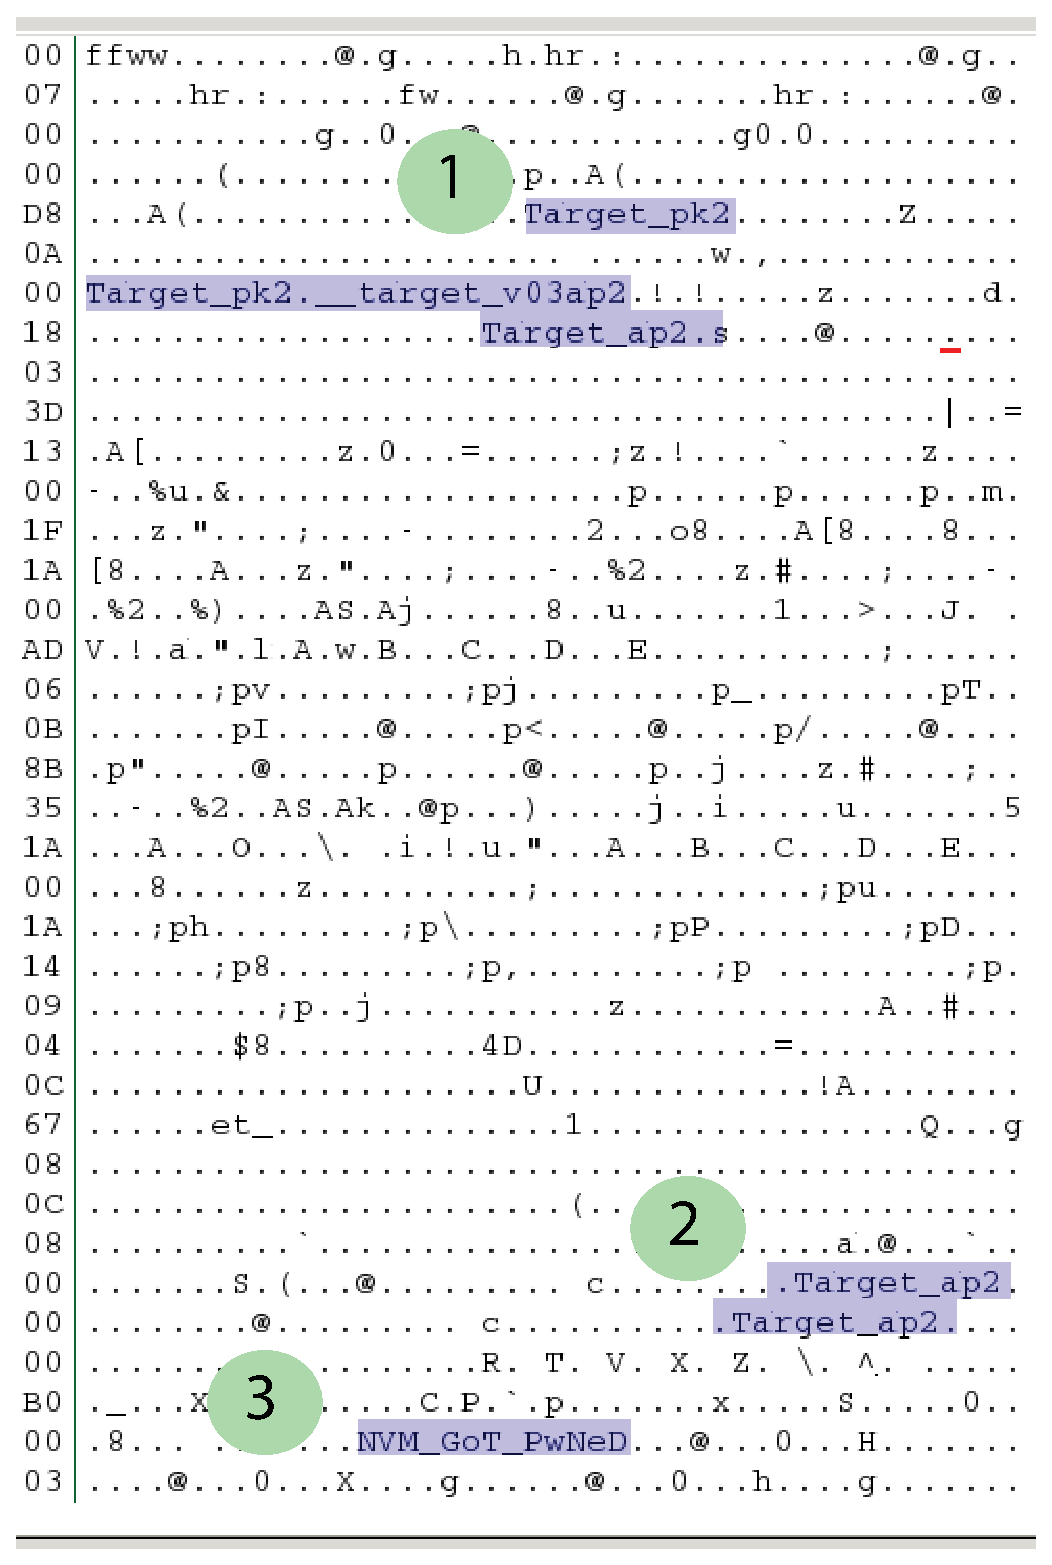
\includegraphics[scale=0.27]{Razafindralambo/img/bless2.eps}
    \caption{Identification of meta-data and a sample of the Non-Volatile Memory area}
    \label{fig:bless2}
\end{figure}
In case of files recovery, there are plenty of file carving tools
\footnote{list of file carving tools: http://forensicswiki.org/wiki/Tools:Data\_Recovery}. The most
known are probably \textit{volatility}, \textit{foremost}, \textit{photorec}.  Most file carvers
operate by simply ``carving out'' blocks after looking for file headers and/or footers. The majority
of file carving programs will only recover files that are not fragmented. 

In practice, while analysing Java Card raw memory dump, one should bear in mind
that the output is platform dependent.  This means that objects, or code
structures, or simply, memory layouts, highly depends on how the Java Card
platform handle them. Therefore, there is no specific structure, or meta-data,
one may always rely on, for automatically identifying the start or the end of the
code. In the example depicted by the Fig. \ref{fig:bless1} one can identify a magic number ($0xDECAFFED$) that identifies the Java Card CAP file format. While in this case it is obvious to determine the start of the applet, this case cannot be generalized on other platforms. However, a trained eye is relatively capable of quickly identifying some
specific details. For instance, a method always ends with a $return$
instruction according to the value to be returned: $return$ (0x7A, return
void), $sreturn$ (0x79, return a short), $areturn$ (0x77, return a reference).
If we still take the same example depicted by the Fig. \ref{fig:bless1}, if one highlights the byte
value $0x7A$ ($return$ instruction), it is possible to distinguish the area where the latter is the
most concentrated.  

\begin{figure}[!h]
\center
    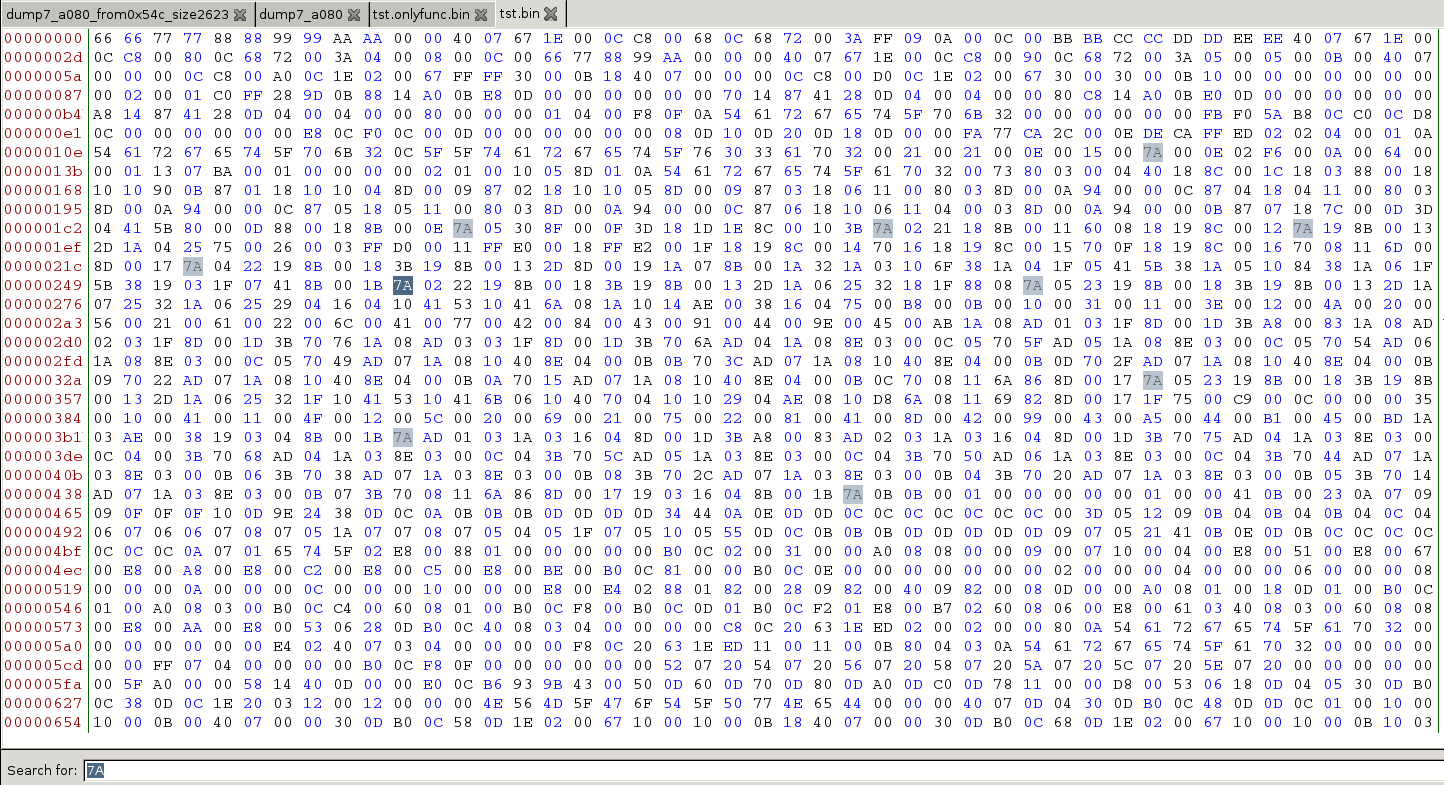
\includegraphics[scale=0.24]{Razafindralambo/img/bless1.eps}
    \caption{Identification of return instructions within a Java Card raw memory dump}
    \label{fig:bless1}
\end{figure}

In this particular example, the methods do not contain that much instructions. Consequently it is relatively easy to highlight the area where the code is located. The larger is the size of the raw memory dump and the different methods, harder is such kind of reverse engineering exercise. Therefore, one must find an automatic way for handling a large raw memory dump, and for distinguishing the code from data. 
%\subsection{Attacks on Java Card Platforms for Dumping the Memory}
%\label{subsection:attacks}
%Several attacks that involve getting read access to some part of smart card's memory have already
%been published. While such kind of attack is not properly detected, this usually leads to dump the
%memory. Getting access to the internal memory allows to gain a better insights for further
%exploitations. In their papers, Witteman in \cite{Witteman} and also Mostowski \textit{et al.}
%in \cite{MostowskiP08} described various type confusion attacks that could lead to an illegal memory
%access. Basically a type confusion attack consists in using an object of type A as an object of type
%B. For instance, a basic type confusion attack that is described in the previous papers is a type
%confusion between a byte array and a short array. Getting access to a byte array as if it is a short
%array would lead to an array overflow during the access if any boundaries checks are properly done.

%\cite{barbu1}
%\cite{heaphop}
%\cite{BouffardForensic}
\subsection{Memory Forensics of a Java Card Dump}
\label{subsection:memforensics}
Bouffard \textit{et al.} described in \cite{conf/cardis/LanetBLCMMF14} a technique that
 uses the Index of Coincidence as a heuristic in order to determine the area in a memory dump that
 is likely to be similar to a Java Card application code.
 The Index of Coincidence basically shows how the frequency distribution of a set A is similar to a
 set B. It is usually used in cryptography for breaking substitution ciphers. For instance, it
 measures how alike cryptogram frequencies are to a given language (e.g: English). In their paper,
 Bouffard \textit{et al.}  state that an acceptable IC for Java Card language is located between
 0.020 and 0.060.  In order to locate Java Card code, they use a sliding window with a certain size,
 that compute an IC value while parsing the memory dump.
However, they do not precise among which kind of byte code they performed their study phase.
Furthermore, they also do not give any information regarding the size/number of samples they used to
determine the proper IC. The more samples are used, the more accurate should be the IC value.


\begin{figure}[!h]
\center
    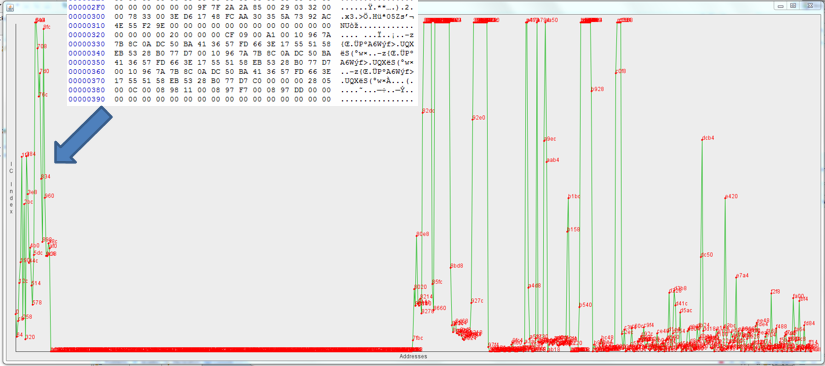
\includegraphics[scale=0.35]{Razafindralambo/img/ic-technique.png}
    \caption{Index of Coincidence computation trace (x-axis: offsets in the memory dump, y-axis: IC values)}
    \label{fig:ic-technique}
\end{figure}
The Fig. \ref{fig:ic-technique} depicts the resulting trace after computing the Index of
Coincidence values over a memory dump using a sliding window. Different area of interest can be noticed. The first one on the leftmost is the
one that contains the actual code. The area of peaks in middle of the graph are just noises. And the
third area does not reflect Java Card code because the width of the multiple blocks that compose this
area are too small.

Over 64Kbytes of memory dump, it appears then that only 380 bytes are necessary and can be considered as
potential Java Card code, so it can be extracted/analysed/disassembled later on.  Once the block
extracted, additional analysis must be performed in order to retrieve the real start of the code
area, and also its real end (dynamic analysis of the control flow graph,
execution/simulation/analysis of the stack, etc.)

\subsection{Visual Reverse Engineering of Binary and Data Files}
\label{subsection:visualreverse}

In their paper Conti \textit{et al.} \cite{Conti:2008:VRE:1431913.1431914} present some design
principles for files analysis. By using different graphing techniques, they show how to identify the
contents of binary files.  Indeed, they demonstrate how quick you can detect certain patterns within
the binary file. This way, it is easier to highlight what is contained within the file. One can notice then that every type
of document (jpg, word, etc.) has its own ''visual signature`` (see figure Fig.\ref{fig:re}). Their results
indicate that visual approaches help analysts for identifying files or analyzing unfamiliar file
structures. These principles are the main essence that led me to follow their approaches.

\begin{figure}[!h]
\center
    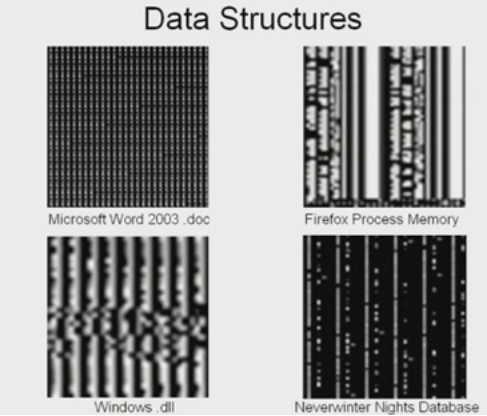
\includegraphics[scale=0.45]{Razafindralambo/img/re.png}
    \caption{Visual signature of (from left to right): a Word document, a Firefox process Memory, a Windows dll, a
    Neverwinter Nights Database}
    \label{fig:re}
\end{figure}






\section{Experiments}
\label{section:exp}
Inspired from Conti \textit{et al.} work \cite{Conti:2008:VRE:1431913.1431914} one can check how CAP
files look like by using one of their graphing technique, in order to check if it is possible to
distinguish the code from the data. During the different tests I have
performed, I worked with Java Card applets that are different in size, and also
in purpose. The first one, named TargetApp, is an application that I have
installed on a given smart card that we will name TargetCard. The loading keys
of the latter were known, that is why I could authenticate and load TargetApp
on the device. The others are just different Java Card applications found on the
internet \footnote{https://github.com/martinpaljak/AppletPlayground}:
JavaCardApp1 (PKIApplet) and JavaCardApp2 (OpenPGPApplet).  The memory dump
used for experiments in the rest of the paper comes from the Non-Volaile Memory
(NVM) area. I successfully dumped the NVM using a malicious ill-formed applet
as presented in \cite{cardis15}. After some static/manual reverse engineering,
I retrieved the code of TargetApp. The aim of the different experiments is then
to try to find a way to perform the previous job (almost)
automatically in order to speed up the reverse engineering step during an evaluation.




\subsection{Visual Signature of a Java Card Application}

As an example I took two different applications and I applied the ``\textit{Byte
Plot}'' technique to visualize their representation, depicted in Fig. \ref{fig:bp1} and Fig. \ref{fig:bp2}.

Fig. \ref{fig:byteplot11} shows how Byte Plots are drawn. The ``Height'' value can be
arbitrarily set and enables define the output size of the image. According to size of image,
patterns can be better spotted. 
\begin{figure}[!h]
\center
    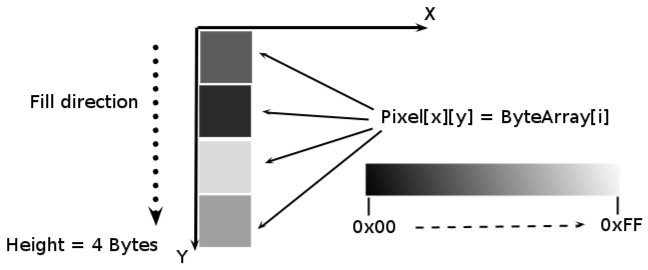
\includegraphics[scale=0.4]{Razafindralambo/img/byteplot11.png}
    \caption{Byte Plot of a byte array.}
    \label{fig:byteplot11}
\end{figure}

\begin{figure}[!h]
    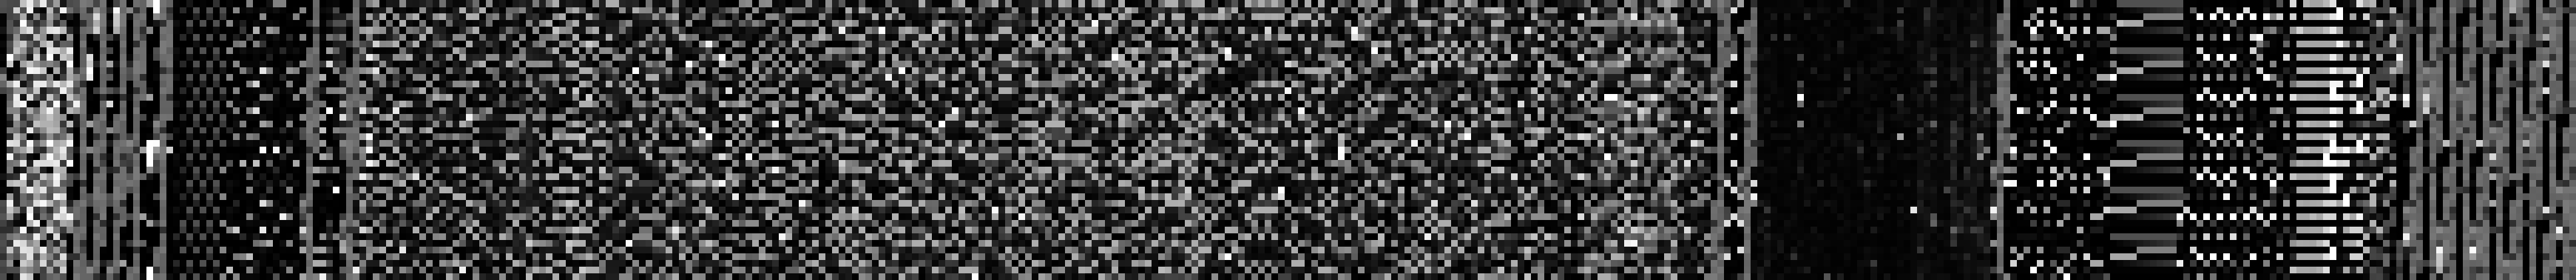
\includegraphics[width=\textwidth]{Razafindralambo/img/hugeapp.png}
    \caption{Visual signature of Java CardApp1 , size = 16KB}
    \label{fig:bp1}
\end{figure}


\begin{figure}[!h]
    \center
    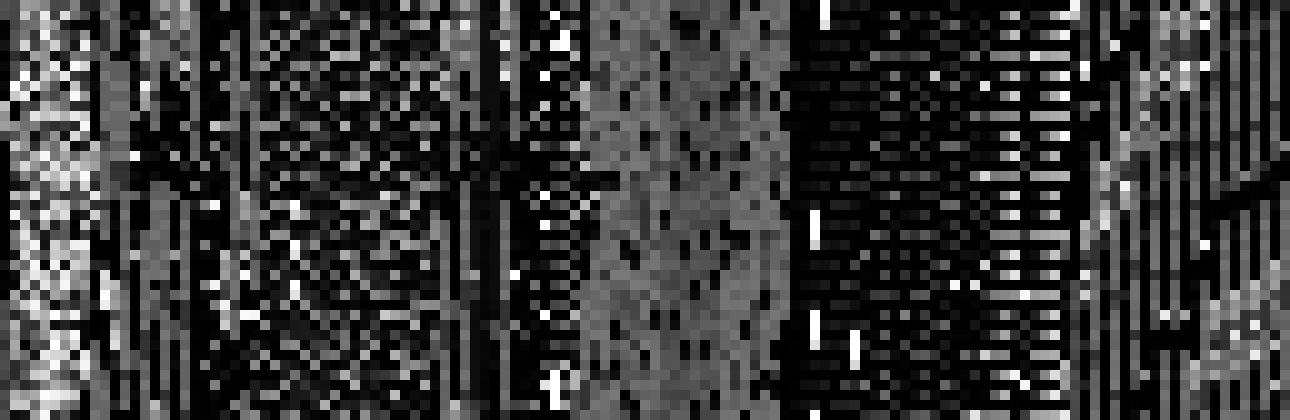
\includegraphics[scale=0.13]{Razafindralambo/img/target.png}
    \caption{Visual signature of a TargetApp, size = 8KB}
    \label{fig:bp2}
\end{figure}

\subsection{CAP components extraction}
A CAP file behaves like a JAR/ZIP archive file format. For instance one can use the software
``\textit{Unzip}'' to extract its content. Once extracted, one can retrieve the different CAP file
components.
%\\
%\dirtree{%
    %.1 myapplication/.
    %.2 javacard/.
    %.3 Header.cap.
    %.3 Directory.cap.
    %.3 Applet.cap.
    %.3 Import.cap.
    %.3 ConstantPool.cap.
    %.3 Class.cap.
    %.3 Method.cap.
    %.3 StaticField.cap.
    %.3 ReferenceLocation.cap.
    %.3 Export.cap.
    %.3 Descriptor.cap.
    %.3 Debug.cap (Optional).
%}

%\paragraph*{}
Once Java CardApp1 (Fig. \ref{fig:bp1}) has been decompressed one can independently draw and check the ``Byte
Plot'' for each CAP file components. For example, below are the plots of the Method component, the
Reference Location and the Descriptor component:

\vspace{-3em}
\begin{figure}[!h]
\begin{center}
\[\arraycolsep=5pt\def\arraystretch{2}
\begin{array}{ccc}
Method & Ref. Location & Descriptor  \\    
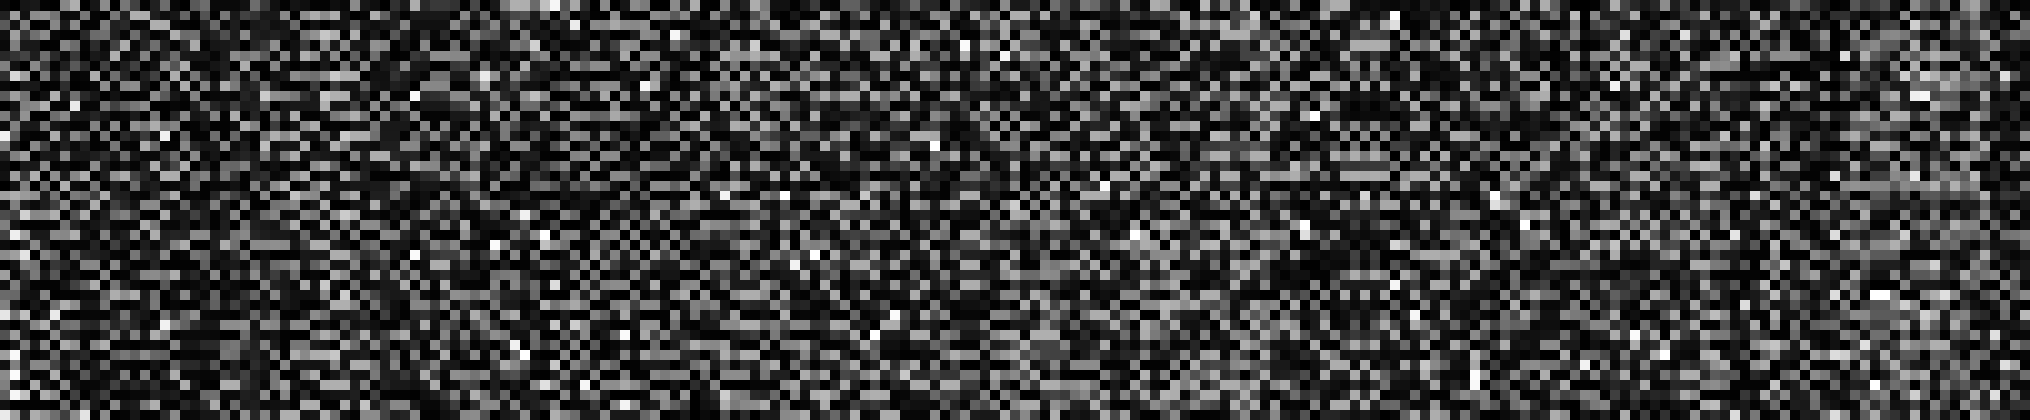
\includegraphics[scale=0.12]{Razafindralambo/img/Method1.png} &
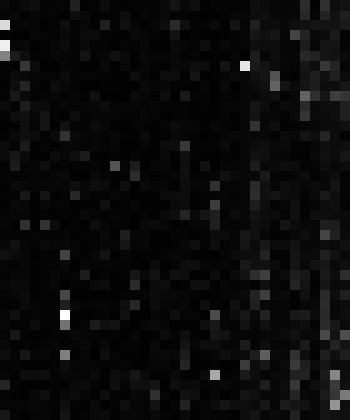
\includegraphics[scale=0.12]{Razafindralambo/img/RefLocation1.png} & 
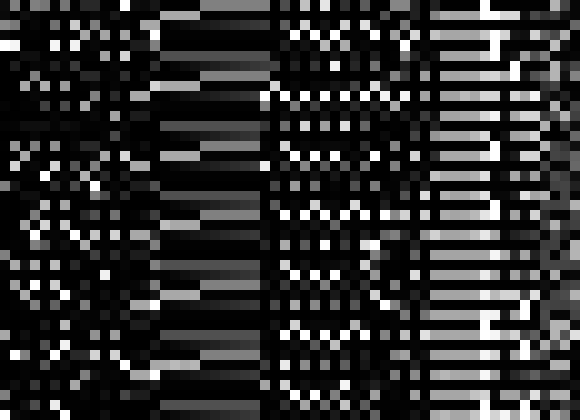
\includegraphics[scale=0.12]{Razafindralambo/img/Descriptor1.png} 
\end{array}
\]
\caption{Byte plots of three specific CAP file components}
\label{fig:bpcompo}
\end{center}
\end{figure}

\vspace{-3em}
\subsection{Byte distributions analysis and characterization}
\subsubsection{Byte distributions --}
What we can deduce from the figures Fig. \ref{fig:bp1}, Fig. \ref{fig:bp2}, Fig.
\ref{fig:bpcompo} is the fact that the code of an application (stored in the Method Component) has a
byte distributions different from the other data that compose a Java Card application. Fig. \ref{fig:bd1} shows a comparison between the byte distributions of different CAP
components (Method component included). Furthermore, one can see in figure Fig. \ref{fig:bd3}
the byte distributions of 8 Method Components from 8 different Java Card applications. 

\begin{figure}[!h]
\begin{center}
\[\arraycolsep=5pt\def\arraystretch{2.1}
\begin{array}{cc}
Java CardApp1 & TargetApp  \\    
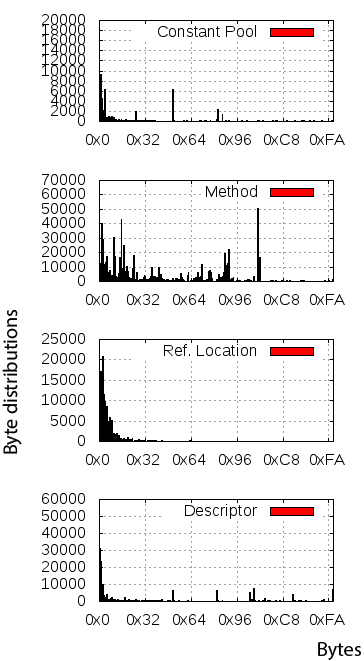
\includegraphics[scale=0.36]{Razafindralambo/img/dist_capcompo_hugeapp.png} &
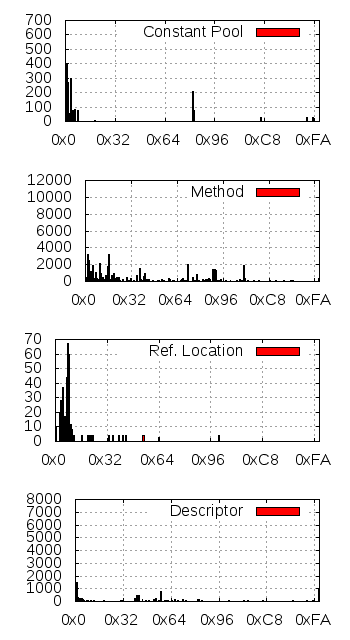
\includegraphics[scale=0.378]{Razafindralambo/img/dist_capcompo_target.png} 
\end{array}
\]
\caption{comparison of byte distributions within 4 components of 2 different applications}
\label{fig:bd1}
\end{center}
\end{figure}

\begin{figure}[!h]
    \center
    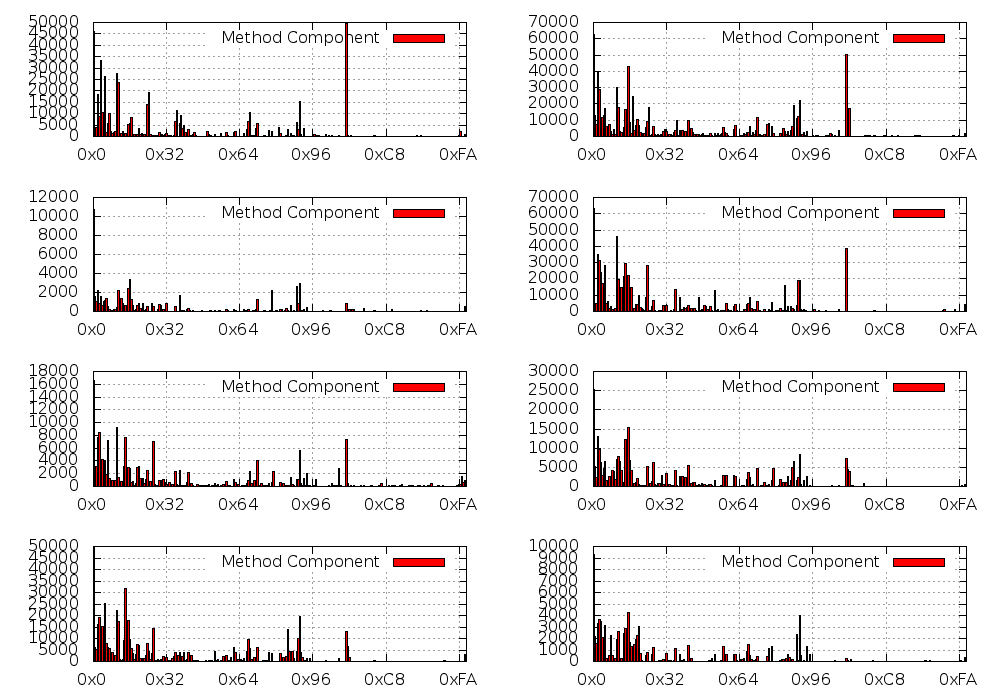
\includegraphics[scale=0.31]{Razafindralambo/img/methodcomponents_dists.png}
    \caption{Byte distributions of different Method Components}
    \label{fig:bd3}
\end{figure}

%\subsubsection{Standard Deviation --}
%\label{subsub:std}
%The standard deviation enables to measure the amount of variation/dispersion of a set of data
%values. Higher the STD value is, wider is the range of values over which one the different
%points are spread out.
 
%If we compare the STD value of a method component and the STD value of other components, we can
%notice that it is way higher while it is computed for the method component as one can see in the
%Table \ref{table:std1}.

%\begin{center}
%\begin{tabular}{c|c|c|c|c|}
    %\cline{2-5}
    %& \multicolumn{4}{ c| }{Standard Deviation values} \\ \cline{2-5}
    %& Cst. Pool & Method & Ref. Loc. & Desc. \\ \cline{1-5}
    %\multicolumn{1}{ |c| }{\multirow{1}{*}{TargetApp}} &
    %\multicolumn{1}{ |c| }{\cellcolor{gray!30} 1494.56} & \cellcolor{red!30}7510.99 & \cellcolor{gray!30}2240 & \cellcolor{gray!30}4345.1 \\ \cline{1-5}
    %\multicolumn{1}{ |c| }{\multirow{1}{*}{Java CardApp1}} &
    %\multicolumn{1}{ |c| }{\cellcolor{gray!30}56.7596} & \cellcolor{red!30}879.129 & \cellcolor{gray!30}7.19022 & \cellcolor{gray!30}506.785 \\ \cline{1-5}
%\end{tabular}
    %\captionof{table}{Standard Deviation values comparison}
    %\label{table:std1}
%\end{center}

%One can notice that the standard deviation value is way higher in the method component area. 

\subsubsection{Statistical tests for comparing two sets of byte distributions --}
As all is a matter of byte distributions, I needed to find a way to test the byte distributions of a
given sample of raw memory dump against a kind of ``template''. This template can be for instance the byte
distributions of the Method Component of another CAP file.

Let $A$ be the byte distributions of a given Method Component, and $B$ a sample of the byte
distributions from the raw memory dump. Furthermore, let $C$ be the byte distributions of another
CAP component. The statistical test is noted $ST$ and $X$, $Y$ are two arbitrary samples of byte
distributions.  The latter should be able to verify the following properties: $ST(A,B) \approx 1$,
$ST(C,B) \approx 0$, $0 \leq ST(X,Y) \leq 1$.
$A$ is a reference that will be compared to $B$. The statistical test should be able to check if $A$
looks like $B$. It should also verifies that, $C$ does not look like $B$.  
choosing the right test to compare two measurements is a bit tricky, as one must choose between two
families of tests: parametric and non-parametric.
Tests are referred to as parametric tests while the data are sampled from a ``\textit{Gaussian}'' or
``\textit{normal}'' distribution. Otherwise if one does not want to make any assumptions regarding
the data distribution one should choose non-parametric tests. 

%The following book \textit{\usebibentry{biostatistics}{title}}, \cite{biostatistics} is an excellent
%introduction to a wide range of statistics notions with a focus on practical applications. The
%chapter 37, titled ``\textit{Choosing a Test}'' is specifically very interesting. It particularly
%explain why/how to choose between parametric and non-parametric tests. 
%The easy cases are when you are definitely sure that your distribution does not follow a
%Gaussian/Normal distribution. That is the trace is approximately bell shaped . In these cases one
%must choose non-parametric statistical tests (which is my case). In the hard cases, it is harder to
%define if a distribution is Gaussian/Normal or not.  In theses cases one can try to use a ``formal
%statistical test'' (e.g: Kolmogorov-Smirnoff test, or Anderson-Darling test) to determine if the
%distribution of the data differs significantly from a Gaussian/Normal distribution.

%\subsubsection{What non-parametric statistical test to choose?}

%In my cases if we take a look at the byte distributions of the different CAP Components from two
%different applets (see Fig. \ref{fig:bd1}) one can notice that is definitely not a Gaussian/Normal
%distribution. Therefore non-parametric statistical tests shoudl fit better my needs.
%From Wikipédia \footnote{http://en.wikipedia.org/wiki/Nonparametric\_statistics\#Methods}, here is a list of non-parametric statistical methods that exist:

%\begin{center}
    %\begin{tabular}{|p{4cm}|p{10cm}|}
    %\hline
    %Methods & Used for \\ \hline
    %Anderson-Darling & tests wether a sample is drawn from a  given distribution \\ \hline 
    %Statistical Bootstrap Methods & estimates the accuracy/sampling distribution of a statistic \\
    %\hline
    %Cochran's Q & test whether \textit{k} in randomized block designs with 0/1 outcomes have
    %identifical effects \\ \hline
    %Cohen's kappa & measures inter-rater agreement for categorical items \\ \hline
    %Friedman 2-way analysis of variance by ranks & tests whether \textit{k} treatments in randomized
    %block designs have identical effects \\ \hline
    %Kaplan-Meler & estimates the survival function from lifetime data, modeling censoring \\ \hline
    %Kendall's Tau & measures statistical dependence between two variables \\ \hline
    %Kendall's W & measure between 0 and 1 of inter-rater agreement \\ \hline
    %Kolmogorov-Smirnov & tests whether a sample is drawn from a given distribution, or whether two
    %samples are drawn from the same distribution \\ \hline
    %Kruskal-Wallis 1-way analysis of variance by ranks & tests whether 2 (or more) independent samples are
    %drawn from the same distribution \\ \hline
    %Kuiper's test & tests whether a sample is drawn from a given distribution, sensitive to cyclic
    %variations such as a day of the week \\ \hline
    %Logrank test & compares survival distributions of two right-skewed censored samples \\ \hline
    %Mann-Whitney U or Wilcoxon rank sum test & tests whether two samples are drawn from the same
    %distribution as compared to a given alternative hypothesis \\ \hline
    %McNemar's test & tests whether, in 2 x 2 contingency tables with a dichotomous trait and matched
    %pairs of subjects, row and column marginal frequencies are equal \\ \hline
    %Median test & tests whether two samples are drawn from distributions with equal medians \\
    %\hline
    %Pitman's permutation test & a statistical significance test that yields exact \textit{p} values
    %by examining all possible rearrangements of labels \\ \hline
    %Rank products & detects differentially expressed genes in replicated microarray experiments \\
    %\hline
    %Siegel-Tukey & tests for differences in scale between two groups \\ \hline
    %Sign test & tests whether matched pair sampels are drawn from distributions with equal medians
    %\\ \hline
    %Spearman's rank correlatino coeff. & measures statistical dependence between two variables using
    %a monotonic function \\ \hline
    %Squared ranks test &  test equality of variances in two or more sampels \\ \hline
    %Wald-Wolfowitz runs test & tests whether the elements of a sequence are mutualy
    %independent/random \\ \hline
    %Wilcoxon signed-rank test & tests whether matched pair samples are drawn from populations with
    %different mean ranks \\ \hline
%\end{tabular}
%\captionof{table}{Non-parametric statistical tests}
    %\label{table:stats1}
%\end{center}



\subsection{Analysis of the byte distributions of a Java Card Memory Dump}

In order to confirm that I properly extracted the right portion of memory that normally contains
the target applet's code, I visually compared the byte distributions of TargetApp against the byte
distributions of A. 
    %\item I compared the standard deviation values of both bytes distribution

As one can see from the figure Fig. \ref{fig:bd2} the byte distributions are definitely the same.
This gives us the information that the code installed on the card has not been altered in any way.


%Image produced by doing:
%./dist2.py _target_v03/javacard/Method.cap > target_meth_dist
%./dist2.py tst.onlyfunc.bin > tst_onlyfunc__dist
% ./plot-distribution-original-versus-extracted.sh azerty && feh azerty.png
\begin{figure}[!h]
\begin{center}
\[\arraycolsep=5pt\def\arraystretch{2.1}
\begin{array}{cc}
Orignal Method Component & Extracted Method's Byte codes  \\    
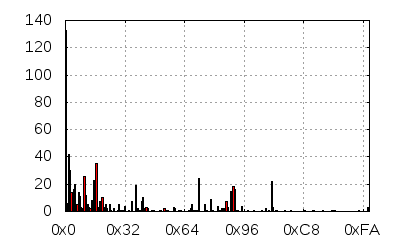
\includegraphics[scale=0.5]{Razafindralambo/img/dist_methcompo_target.png} &
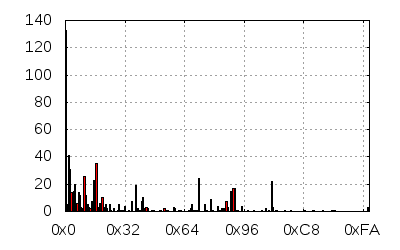
\includegraphics[scale=0.5]{Razafindralambo/img/dist_target_dump_onlyfunc.png} 
\end{array}
\]
\caption{comparison of byte distributions between the original target applet's method component
    (distribution of reference) and the extracted byte codes}
\label{fig:bd2}
\end{center}
\end{figure}

%%\TIANA:  IMAGE PRODUIT AVEC nuages-points.sh
%\begin{figure}[!h]
%\begin{center}
%\[\arraycolsep=-1pt\def\arraystretch{2.1}
%\begin{array}{ccc}
%A\_vs.\_TargetApp\ & A\_vs.\_Java CardApp1 & A\_vs.\_Java CardApp2  \\    
%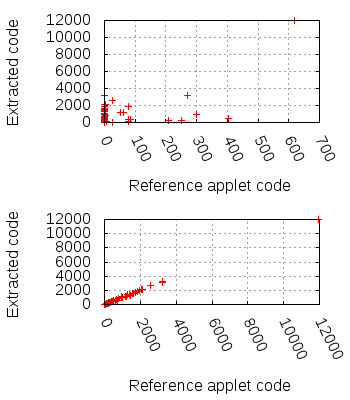
\includegraphics[scale=0.54]{target_vs_dump_plot.png} &
%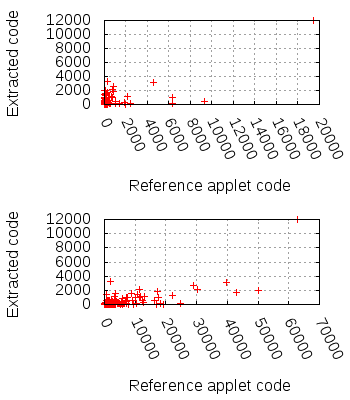
\includegraphics[scale=0.54]{sizzle_vs_dump_plot.png} &
%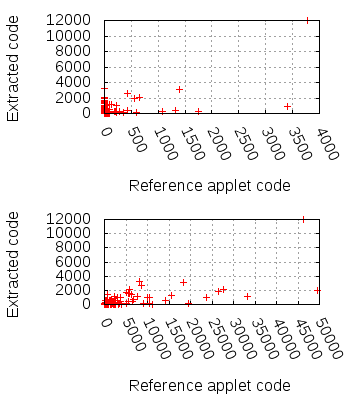
\includegraphics[scale=0.54]{atmpmpc_vs_dump_plot.png}
%\end{array}
%\]
%\caption{Comparison between bytes distributions: X-axis is the byte distribution of the method
%component of an applet of reference, Y-axis is the byte distribution of the code that has been
%extracted. There are 255 points.}
%\label{fig:plot1}
%\end{center}
%\end{figure}

%\paragraph*{Standard deviation} -- 
%They respectively have the following standard deviation value: 879.129 and 879.324.
\vspace{-1em}
\subsubsection{Correlation tests --}

The Pearson Correlation enables to compare two data sets in order to determine if similarities
exist. In our case a data set is represented by  byte distributions.

 As we can see in the Table \ref{table:corr1} the value of the correlation computation while
 we compare the extracted code and the method component of the TargetApp is nearly equal to 1
 (0.999802). 
 If we compare A against the byte distributions of other CAP components (Constant Pool, reference
 Location, Descriptor components), the correlation computation result is lower.
 However, if we perform the same tests against other (totally different) applications (Java CardApp1
 and Java CardApp2, 2nd and 3rd lines) the results do not really help. Indeed, according to the 2nd
 line of the table, the Constant Pool(0.755622), the Method Component (0.7452), and the Descriptor
 Component (0.714169), are all three similar to TargetApp's Method Component, which is obviously not true.
 
 
\begin{table}
\begin{center}
\begin{tabular}{c|c|c|c|c|}
    \cline{2-5}
    & \multicolumn{4}{ c| }{Pearson correlation values} \\ \cline{2-5}
    & Cst. Pool & Method & Ref. Loc. & Desc. \\ \cline{1-5}
    \multicolumn{1}{ |c }{\multirow{1}{*}{TargetApp}} &
    \multicolumn{1}{ |c| }{\cellcolor{gray!30}0.669712} & \cellcolor{red!30}0.999802 &
    \cellcolor{gray!30}0.224208 & \cellcolor{gray!30}0.823772 \\ \cline{1-5}
    \multicolumn{1}{ |c }{\multirow{1}{*}{Java CardApp1}} &
    \multicolumn{1}{ |c| }{\cellcolor{red!30}0.755622} & \cellcolor{gray!30}0.7452 &
    \cellcolor{gray!30}0.270308 & \cellcolor{gray!30}0.714169 \\ \cline{1-5}
    \multicolumn{1}{ |c }{\multirow{1}{*}{Java CardApp2}} &
    \multicolumn{1}{ |c| }{\cellcolor{gray!30}0.652619} & \cellcolor{gray!30}0.699482 &
    \cellcolor{gray!30}0.180559 & \cellcolor{red!30}0.822216 \\ \cline{1-5}
\end{tabular}

\end{center}

\caption{Pearson Correlation values comparison between dumped code and different CAP
    components}
    \label{table:corr1}
\end{table}
    %\captionof{table}{Pearson Correlation values comparison between dumped code and different CAP
    %components}
    

Another interesting statistical tool is the Spearman's rank test. The main difference between
Pearson and Spearman is regarding the evaluation of the relationship between the two data sets to
compare. Pearson will actually evaluate the linear relationship between two data sets, that is, it
expects that one change in A will be associated with a proportional change in B.  However, for
Spearman, it evaluates the monotonic relationship, that is, both A and B can change together but not
necessarily at a constant rate.


\begin{table}
\begin{center}
\begin{tabular}{c|c|c|c|c|}
    \cline{2-5}
    & \multicolumn{4}{ c| }{Spearman (Rho) Ranked Correlation values} \\ \cline{2-5}
    & Cst. Pool & Method & Ref. Loc. & Desc. \\ \cline{1-5}
    \multicolumn{1}{ |c }{\multirow{1}{*}{TargetApp}} &
    \multicolumn{1}{ |c| }{\cellcolor{gray!30}0.3935} & \cellcolor{red!30}0.99762 & \cellcolor{gray!30}0.38933 & \cellcolor{gray!30}0.328617 \\ \cline{1-5}
    \multicolumn{1}{ |c }{\multirow{1}{*}{Java CardApp1}} &
    \multicolumn{1}{ |c| }{\cellcolor{gray!30}0.431883} & \cellcolor{red!30}0.658014 & \cellcolor{gray!30}0.4720988 & \cellcolor{gray!30}0.382773 \\ \cline{1-5}
    \multicolumn{1}{ |c }{\multirow{1}{*}{Java CardApp2}} &
    \multicolumn{1}{ |c| }{\cellcolor{gray!30}0.33328} & \cellcolor{red!30}0.65953 & \cellcolor{gray!30}0.492259 & \cellcolor{gray!30}0.174243 \\ \cline{1-5}
\end{tabular}
\caption{Spearman Ranked Correlation values comparison between dumped code and
    different CAP components}
        \label{table:corr2}
\end{center}
\end{table}
    %\captionof{table}{Spearman Ranked Correlation values comparison between dumped code and
    %different CAP components}


From the Table \ref{table:corr2} one can notice that Spearman Ranked correlation values seem to be
more reliable. Any CAP Components that is not code is under the value $0.5$, otherwise it is above.

 In the same way as Spearman, Kendall's Tau correlation coefficient
uses statistical associations based on the ranks of the data. While Spearman can be thought of as
the regular Pearson product moment correlation coefficient (except it is computed from ranks), on
the other hand Kendall's Tau rather quantifies the difference between the percentage of concordant
(ordered in the same way) and discordant (ordered differently) pairs among all possible pairwise
events.


\begin{table}
\begin{center}
\begin{tabular}{c|c|c|c|c|}
    \cline{2-5}
    & \multicolumn{4}{ c| }{Kendall's Tau values} \\ \cline{2-5}
    & Cst. Pool & Method & Ref. Loc. & Desc. \\ \cline{1-5}
    \multicolumn{1}{ |c }{\multirow{1}{*}{TargetApp}} &
    \multicolumn{1}{ |c| }{\cellcolor{gray!30}0.280127} & \cellcolor{red!30}0.9942593 &
    \cellcolor{gray!30}0.34823 & \cellcolor{gray!30}0.2814312 \\ \cline{1-5}
    \multicolumn{1}{ |c }{\multirow{1}{*}{Java CardApp1}} &
    \multicolumn{1}{ |c| }{\cellcolor{gray!30}0.3777} & \cellcolor{red!30}0.52729 &
    \cellcolor{gray!30}0.41179 & \cellcolor{gray!30}0.30677 \\ \cline{1-5}
    \multicolumn{1}{ |c }{\multirow{1}{*}{Java CardApp2}} &
    \multicolumn{1}{ |c| }{\cellcolor{gray!30}0.295751} & \cellcolor{red!30}0.547625 &
    \cellcolor{gray!30}0.428279 & \cellcolor{gray!30}0.14866 \\ \cline{1-5}
\end{tabular}
\caption{Kendall's Tau values comparison between dumped code and
    different CAP components}
        \label{table:corr3}
\end{center}
\end{table}
   % \captionof{table}{Kendall's Tau values comparison between dumped code and
   % different CAP components}

Now that it is possible to compare two samples of byte distributions, one can use these statistical tools for analysing the whole raw memory dump. 


\section{Automated Java Card Application Code Detection}

While the memory dump to reverse engineer is not too large, a trained eye can manually/statically locate the code. However, in the case where one has a bigger memory dump, an automated
tool would be necessary to highlight the potential area where it appears likely to be code and not
data.

In the previous section I tried to characterize a Java Card applet's code in order to determine a
kind of quantifier that would enable one to determine if a given set of extracted bytes looks more similar to a
code than data. As I have now some statistical tools to rely on, I can use them for identifying
code within a given memory dump, and extract the code.


\subsection{The Running Correlation Coefficient Computation Trace (RCCT)}
The idea is to compare two sets of data, namely, two sets of byte distributions. The first one comes from a reference Java Card applet. Let us note this reference set as $S$. The second set of byte distributions comes from a raw memory dump. While the memory dump is parsed a window of size $w$, is defined for analysing a single sample from the raw memory dump. Let $S_i$ be a given sample where $i$ identifies the sample among other ones. $i$ varies from $0$ to $W/w$, where $W$ is the size of the raw memory dump. While this window is moved from the start of the raw memory dump to its end, every $S_i$ is compared to $S$ using a statistical tool noted ($ST$). The outcome from this computation is a correlation coefficient value $c_i$, that defines how likely $S_i$ is similar to $S$. A set of $c_i$ values will result in a correlation coefficient trace.
For instance, the Fig. \ref{fig:runncorrcoeff} depicts a trace that has been computed while computing $ST(S_i, S)$ all along a raw memory dump, where $w$ has been chosen empirically ($=128$) and $W = 4KB$. 
%TIANA
%./PythonScripts/scan.py tst.bin tst.onlyfunc.bin 42 tst_63x42.png >| spearman_tst.bin_vs_tst.onlyfunc.bin && ./ShellScripts/corrplot.sh spearman_tst.bin_vs_tst.onlyfunc.bin spearman_tst.bin_vs_tst.onlyfunc.bin && feh spearman_tst.bin_vs_tst.onlyfunc.bin.png
\begin{figure}[!h]
    \center
    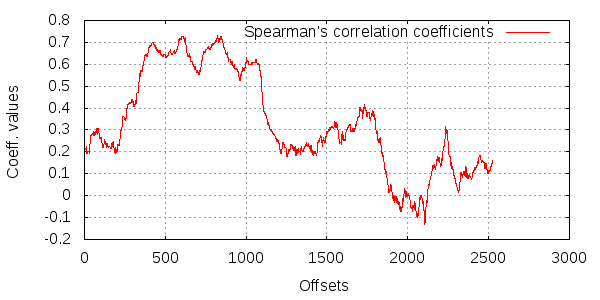
\includegraphics[scale=0.58]{Razafindralambo/img/running_corr_coeff.png}
    \caption{Running Correlation Coefficient Traces}
    \label{fig:runncorrcoeff}
\end{figure}

As we can notice, the correlation coefficient does not even reach 1. This is normal because we do not compare exactly the same thing. However, there is an area between the offsets 470 and $\approx$ 1100, where the correlation coefficient is higher than 0.5. This gives the information that between those offsets, there is a set of bytes that have a distribution that approximate the distribution of the bytes that one can find within the Method Component of the reference Applet that has been chosen for the experiment. Further analysis can reveal which range of window' size can be chosen so the
correlation coefficient is the nearest possible of 1. The Fig. \ref{fig:testwindowsize} depicts a trace where each point represents the number of correlation coefficient that is over 0.9 according to a given window size (absciss).This enables to highlight the range of window size values that can be used for getting the highest correlation coefficient values possible.

%TIANA: produit par ShellScript/corrplot.sh
\begin{figure}[!h]
    \center
    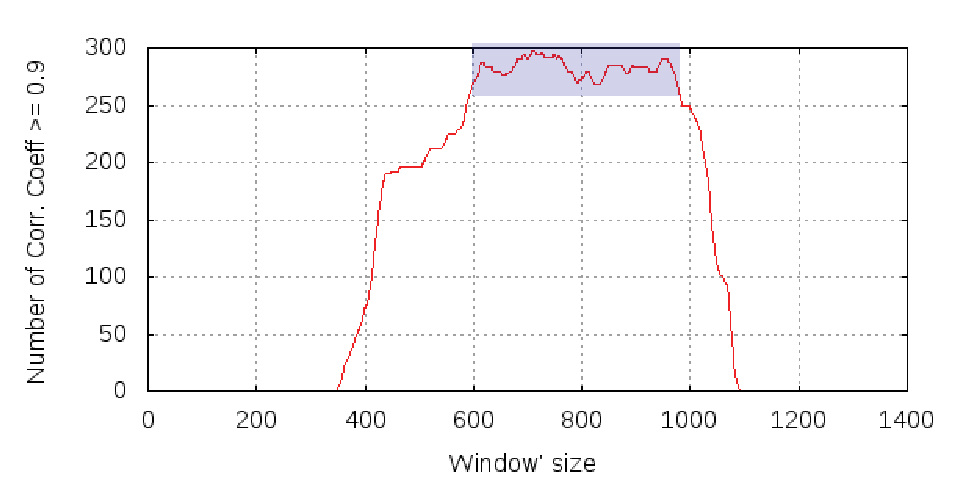
\includegraphics[scale=0.58]{Razafindralambo/img/testwindowsize.eps}
    \caption{Number of Correlation Coefficient greater or equal to 0.9 according to
    the window' size over 2653 bytes}
    \label{fig:testwindowsize}
\end{figure} 

Indeed, 
as one can notice in Fig. \ref{fig:testwindowsize}, the correlation coefficient value is quite high between the offsets 600 and 800 (window'
size). Hence, if one recomputes the correlation trace, one can notice that the area of interest can
be refined (Fig. \ref{fig:window700}).

%TIANA: produit par ShellScript/corrplot.sh
%/PythonScripts/scan.py tst.bin tst.onlyfunc.bin 42 tst_63x42.png > a.txt
%./ShellScripts/corrplot.sh a.txt a.txt  && feh a.txt.png
%a.txt.png ~/Thesis/Javacard_forensics/rcc_window700.png 
\begin{figure}[!h]
    \center
    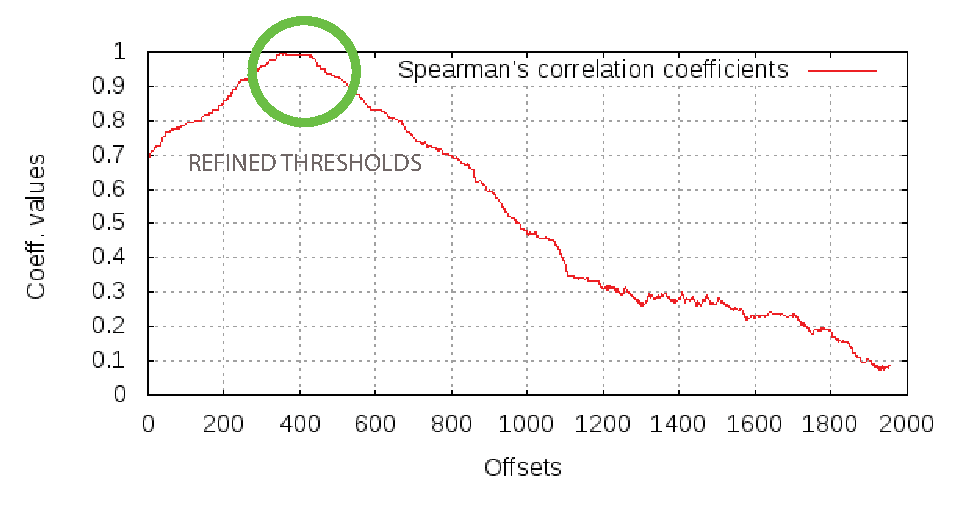
\includegraphics[scale=0.58]{Razafindralambo/img/rcc_window700.eps}
    \caption{Correlation Coefficient computation with a window' size equals to 700}
    \label{fig:window700}
\end{figure}

%\subsection{Data Extraction: the Min/Max Threshold Way}
%After computing the Running Correlation Coefficient computation, according to the values of the
%coefficients, one can define a ``min/max threshold'' in order to delimit the area to extract. The
%problem is that the result of the Running Correlation Coefficient computation is highly dependent to
%the size of the window that has been chosen.

%In order to have the best RCCT trace, one should perform a learning phase. During the latter one
%should compute the RCCT several time with different window' size. 

%The trace that has the highest correlation coefficient values is likely the best one to use as a
%reference to extract the corresponding area in the memory dump.

\subsection{Data Extraction}
A RCCT trace can be used for defining the area of interest to extract. A min/max threshold can be
then used to accomplish that job.
However, I decided to check visually what looks like a RCCT trace while it is plotted as an image instead of
a graph. This would give another way to visually appreciate the variations.

To do so, I defined the color of a pixel as being the absolute value of the correlation coefficient
value that has been rounded up. I kept the gray-scale mode so it is more convenient to process the
image. Therefore as a pixel is defined by its RGB values (Red, Green, Blue).


The resulting image is depicted by the figure Fig. \ref{fig:imgrunncorrcoeff}.

\begin{figure}[!h]
\begin{center}
    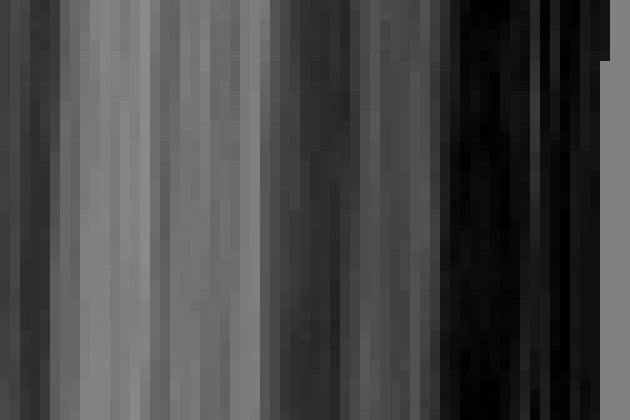
\includegraphics[scale=0.2]{Razafindralambo/img/imgrunncorrcoeff.png}
    \caption{Running Correlation Coefficient plots}
    \label{fig:imgrunncorrcoeff}
\end{center}
\end{figure}

What we can notice is that, the lighter the colour is, the higher the correlation is. It clearly
defines some more visible area . But we need a more accurate delimitation. The gray section on the
rightmost is an ignored part due to the window size.

From the previous image (cf. figure Fig. \ref{fig:imgrunncorrcoeff}) I needed to create a ``mask''
that would enable me to extract from the original raw image the area that
interests me.

Let us say an image is represented as a multidimensional array of RGB values (pixels) such as:
 
image = [ [$R_1$, $G_1$, $B_1$],
          ...  ,
          [$R_n$, $G_n$, $B_n$] ]
 

To create my mask I just defined it such as, every pixel's value greater than the mean value of the
flattened multidimensional array will be set as ``white'' , otherwise it is set to
``black''. 

The result is the figure Fig. \ref{fig:mask1}.
\begin{figure}[!h]
\begin{center}
    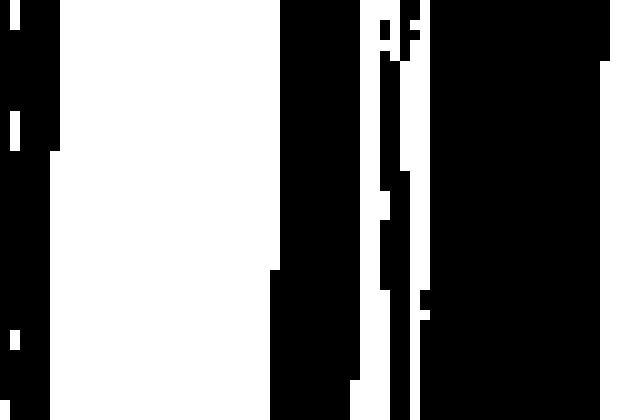
\includegraphics[scale=0.2]{Razafindralambo/img/mask.png}
    \caption{Mask processed from Fig. \ref{fig:imgrunncorrcoeff}}
    \label{fig:mask1}
\end{center}
\end{figure}

Last but not least, I just overlap my brand new mask over the memory dump and I only extract
pixels that actually overlap pixels that correspond to the white color. All the
transformations are summarized by the figure Fig. \ref{fig:extract1}.

\begin{figure}[!h]
\begin{center}
    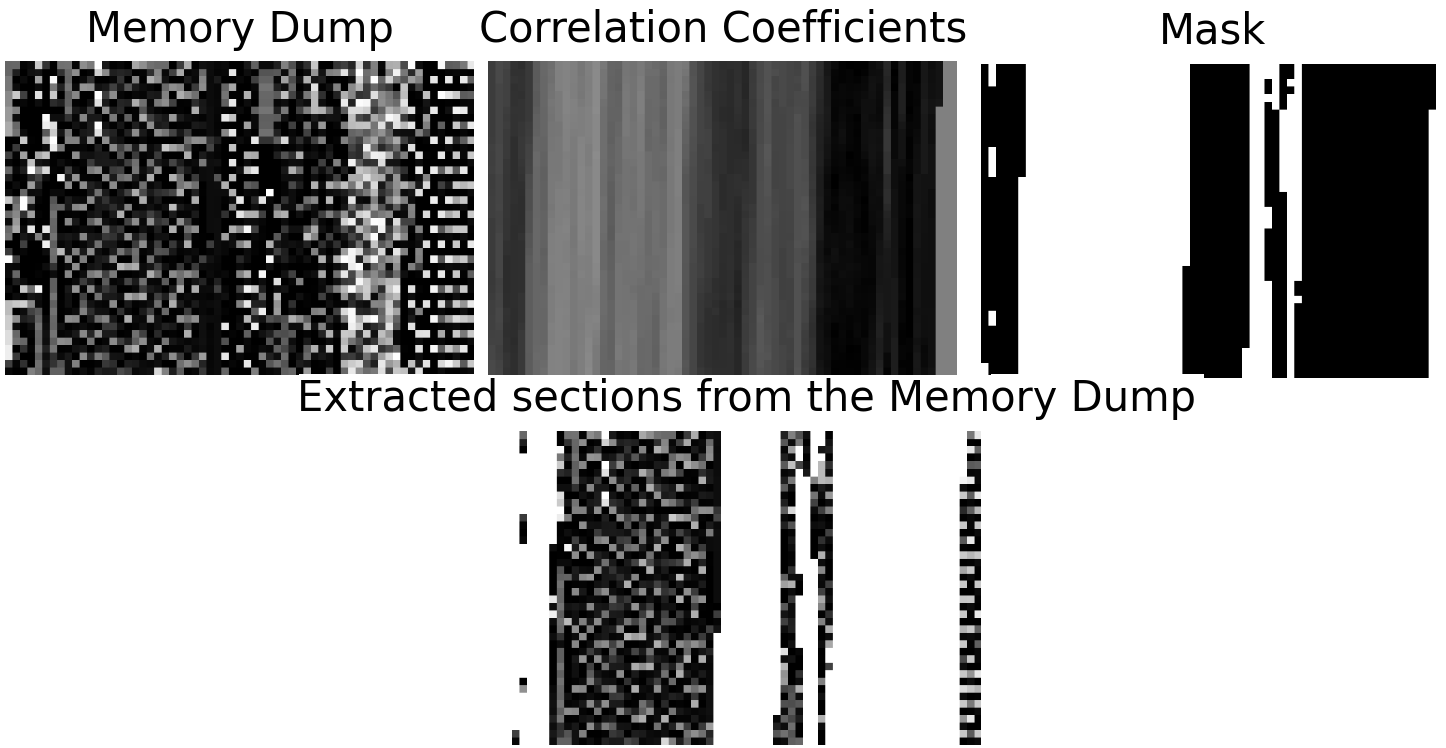
\includegraphics[scale=0.21]{Razafindralambo/img/img_processing.png}
    \caption{Image processing steps for extracting relevant blocks}
    \label{fig:extract1}
\end{center}
\end{figure}
In this example it is easy to decide/choose the right block to select. The small blocks on the left
and the ones  just after the big one cannot be code because an actual method component cannot be
that small or too fragmented. The rightmost block corresponds to the last part that has been left
due to the size of the window during the running correlation coefficient computation.  It remains
the biggest block. 

Once extracted from the raw memory dump, it turns out that due to the sliding window's size, the
beginning and the end of the method component is actually not properly delimited. It may remain some
bytes before and after the extracted data that are not related to the code. They can be easily
identified while we try do decompile the extracted data due to incoherences in the code's semantic.
%\section{Countermeasures}

%As one can notice from the previous anlysis, a byte distributions analysis might characterize an area that represent code.
%Everything is a matter of frequency occurences. An interesting study to make would be a comparison
%of the byte distributions of a set of codes that have been obfuscated. It would be interesting to
%determine if some obfuscation techniques can actually be defeated due to a pattern that can be
%noticed through the visual signature of the code. Such pattern implies that a statistical analysis
%can characterize the resulting obfuscated code. 

%A good countermeasure would be then an obfuscation technique that does not enable to perform any
%statistical analysis on the resulting code.

%\section{Countermeasures} 
%The only countermeasure to this is to break the code into multiple small blocks instead of having a
%huge block of code that is easier to retrieve.

\section{Countermeasures}

This technique has a strong reliability just because of one fact: the Method Component (meta-data +
methods' body) and/or a set of grouped methods' body  has a very specific byte distributions compared
to other CAP components (or other non-related data or meta-data that surround the code). However, countermeasures already exists as addressed in \cite{barbuthesis}
\cite{dynamicsyntax}. 

\subsection{Instructions Scrambling}
The first countermeasure just consists in scrambling the Java Card instruction set. To do so, each
instructions are XORed with a randomly generated byte. 
 
 \begin{center}
scrambled\_instruction = original\_instruction $\oplus$ KEY 
\end{center}

Consequently, two devices can then have two different instruction sets. As the instruction set is
unknown to the attacker, this is enough to circumvent the different analysis that have been
proposed in this paper.

However, as it as been noted in \cite{dynamicsyntax} the XOR key can be revealed. First of all, if
an attacker is able to change the control flow of the program to a $return$ instruction or if he is
able to identify its scrambled version, the XOR key can be easily broken by brute-forcing it.
Indeed, the $return$ instruction's value is $0x7A$. Its scrambled version can only take 256 possible
values which is nothing in term of brute-forcing.  
Secondly, if a scrambled instruction is repeated too many times, this can give some hints to the
attacker regarding the real instruction's value. If his assumptions turned to be true, then the same
brute-force attack can be applied.

Hence another countermeasure has been proposed in \cite{dynamicsyntax} and is explained in the next section.

\subsection{Improved Instructions Scrambling}

To improve the above countermeasure, as explained in \cite{dynamicsyntax},in addition to the XOR
key, a dynamic element has been added in order to circumvent the weakness that has been noted
previously. The Java Program Counter is then included in the scrambling operation:
 
 \begin{center}
scrambled\_instruction = original\_instruction $\oplus$ KEY $\oplus$ JPC
\end{center}

In this case every scrambled instructions will have different values.

\section{Conclusion}
This paper described a new approach for identifying and extracting Java Card code from a raw memory
dump. The aim of this work was to find another technique that would overcome the gathering of a wide range of
different applications that is required for computing a proper Index of
Coincidence (IC). As it has been described in \cite{conf/cardis/LanetBLCMMF14}, that IC value should characterize at best the Java Card set of instructions.
Some countermeasures have already been proposed in the literature
\cite{barbuthesis}, \cite{dynamicsyntax} and are efficient enough for
circumventing such kind of analysis. However, in the case the right
countermeasure is not properly set up, the new approach I propose enables to
characterize the code embedded within a Java Card applet. The main characteristic of the code is its byte distributions. It has been shown that using some statistical tools enables to use this characteristic
for distinguishing the code from data. It has also been shown that,
instead of characterizing the whole Java Card programming language, a single
reference sample (a Java Card applet) suffices for the characterization and the
identification steps. This technique thrives on the fact that the Method
Component within a Java Card applet has a particular byte distributions that
can be recognized amongst data that do not have any relation with the latter. This technique enables to speed up the reverse engineering process while one faces a large raw memory dump.

%\section{Future works}
%\paragraph*{01/04/2015} Enhance the characterization step and find other heuristics.
%\paragraph*{03/04/2015} Define which non-parametric statistical tests fit better my needs. Start to think of countermeasures that would enable to
%defeat any statistical analysis on bytes distribution.
%\paragraph*{15/04/2015} Countermeasures? Analsysis of obfuscation's effects? Analysis of other
%family of bytecodes?



\bibliographystyle{plain}
\bibliography{Razafindralambo/biblio}

\end{document}
